На основе значения коэффициента вариации \(CV\), рассчитанного для различных подвыборок, было выбрано распределение, аппроксимирующее заданную случайную последовательность:

\begin{itemize}
	\item Для подвыборок с количеством случайных величин 10, 20, 50, 100, 200 и 300 значения коэффициента вариации составляют \(33.389\%\), \(46.491\%\), \(60.786\%\), \(66.043\%\), \(69.558\%\), и \(69.986\%\) соответственно.
	\item Так как все значения коэффициента вариации находятся в диапазоне \(0 < CV < 100\%\), было выбрано \textbf{нормированное распределение Эрланга k-го порядка} для аппроксимации закона распределения. Это распределение подходит для данных с коэффициентом вариации ниже \(100\%\), где распределение менее дисперсно по сравнению с экспоненциальным.
\end{itemize}

Функция плотности вероятности для распределения Эрланга k-го порядка имеет вид:

\[
	f(x; k, \lambda) = \frac{\lambda^k x^{k-1} e^{-\lambda x}}{(k-1)!}
\]
где \(k\) — порядок распределения, \(\lambda\) — параметр, обратный среднему значению.

Например, для различных $k$ и $\lambda$ распределения Эрланга может принимать следующий вид (Рис. 5). Чтобы понять какой характерен нашей ЧП, надо произвести расчёт параметров для распределения Эрланга.

\FloatBarrier
\begin{figure}[h]
	\centering
	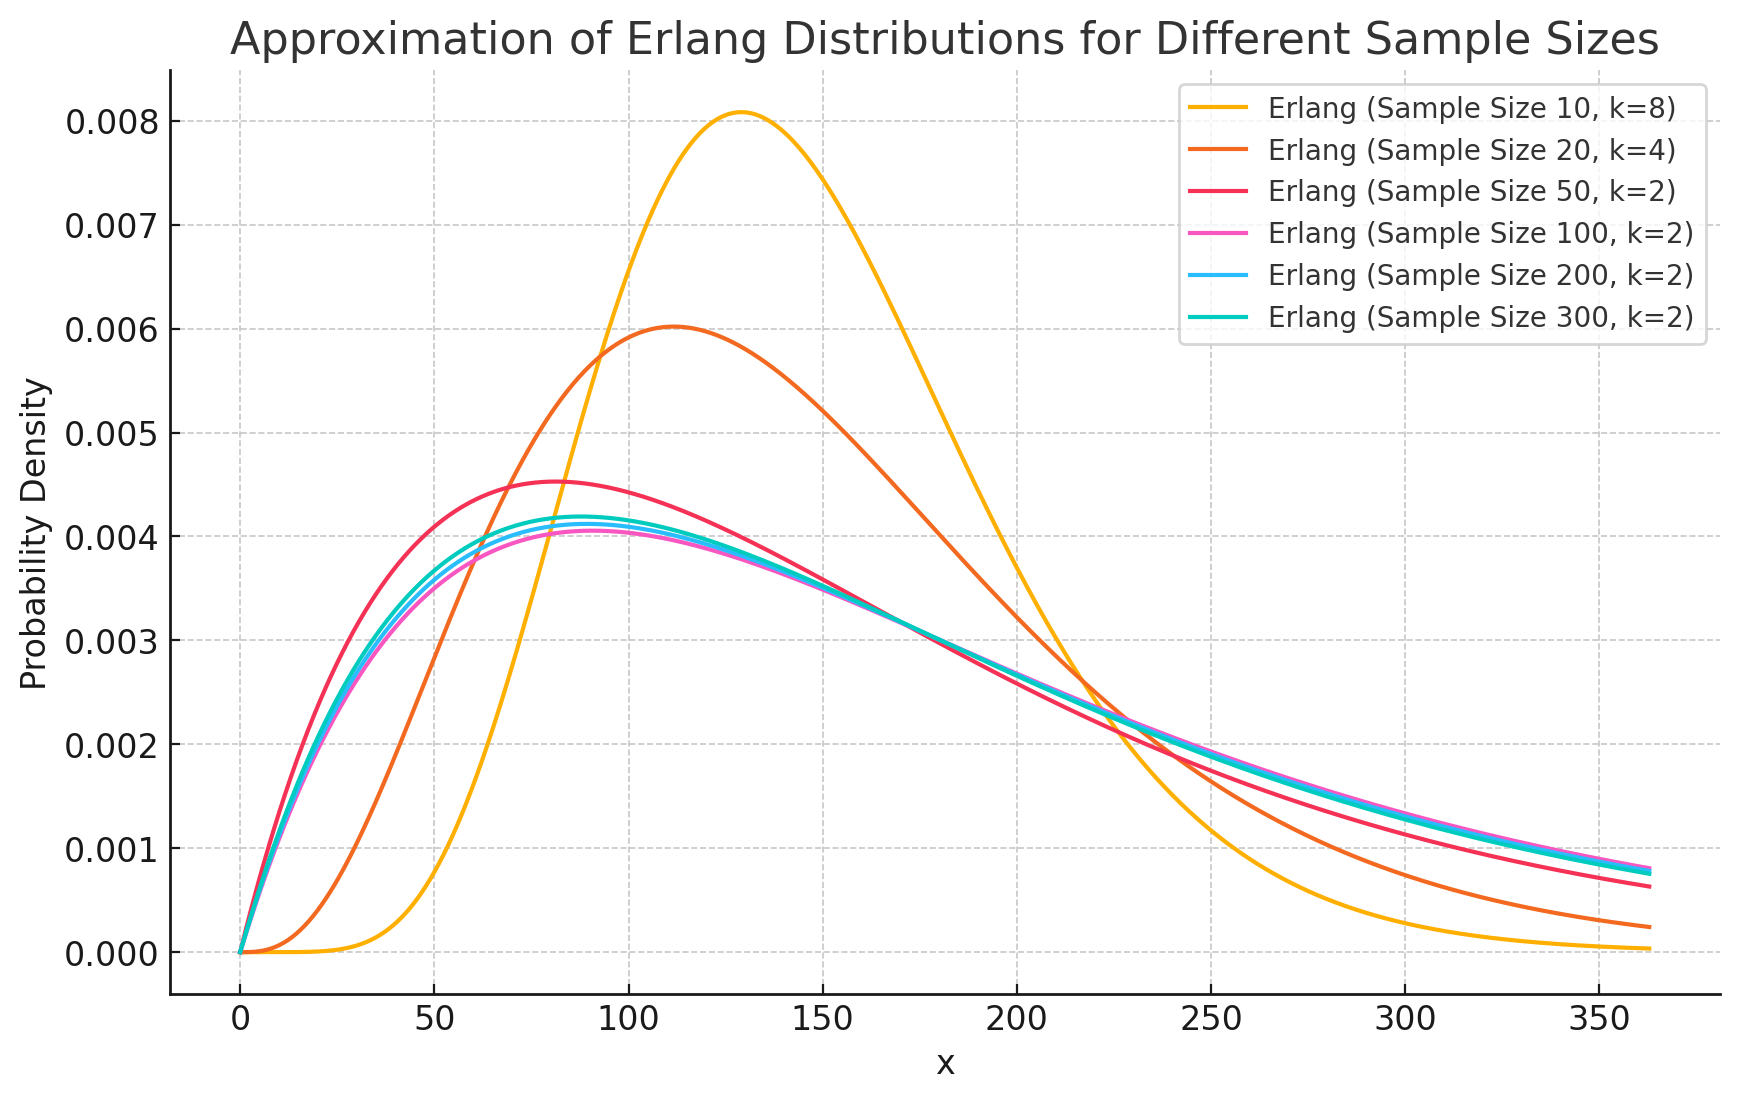
\includegraphics[width=1\textwidth]{../data/histogram_example.png}
	\caption{Распределение Эрланга для различных параметров}
\end{figure}
\FloatBarrier

\subsection{Расчёт параметров распределения Эрланга для ЧП из 300 элементов}

\begin{enumerate}
	\item Для последовательности из 300 элементов у нас есть следующие данные:
	      \[
		      \mu = 175.5133 \quad \text{(математическое ожидание)}
	      \]
	      \[
		      \sigma^2 = 15088.212 \quad \text{(дисперсия)}
	      \]

	\item Теперь мы можем рассчитать порядок \(k\) распределения Эрланга по формуле:
	      \[
		      k = \frac{\mu^2}{\sigma^2}
	      \]
	\item Подставляем значения:
	      \[
		      k = \frac{175.5133^2}{15088.212} = \frac{30714.96}{15088.212} \approx 2.036
	      \]
	\item Округляем до ближайшего целого числа:
	      \[
		      k \approx 2
	      \]

	\item Далее рассчитываем параметр масштаба \( \lambda \) по формуле:
	      \[
		      \lambda = \frac{k}{\mu}
	      \]
	\item Подставляем значения:
	      \[
		      \lambda = \frac{2}{175.5133} \approx 0.0114
	      \]

	\item Таким образом, для последовательности из 300 элементов параметры распределения Эрланга следующие:
	      \[
		      k = 2, \quad \lambda = 0.0114
	      \]

\end{enumerate}


\FloatBarrier
\begin{figure}[h]
	\centering
	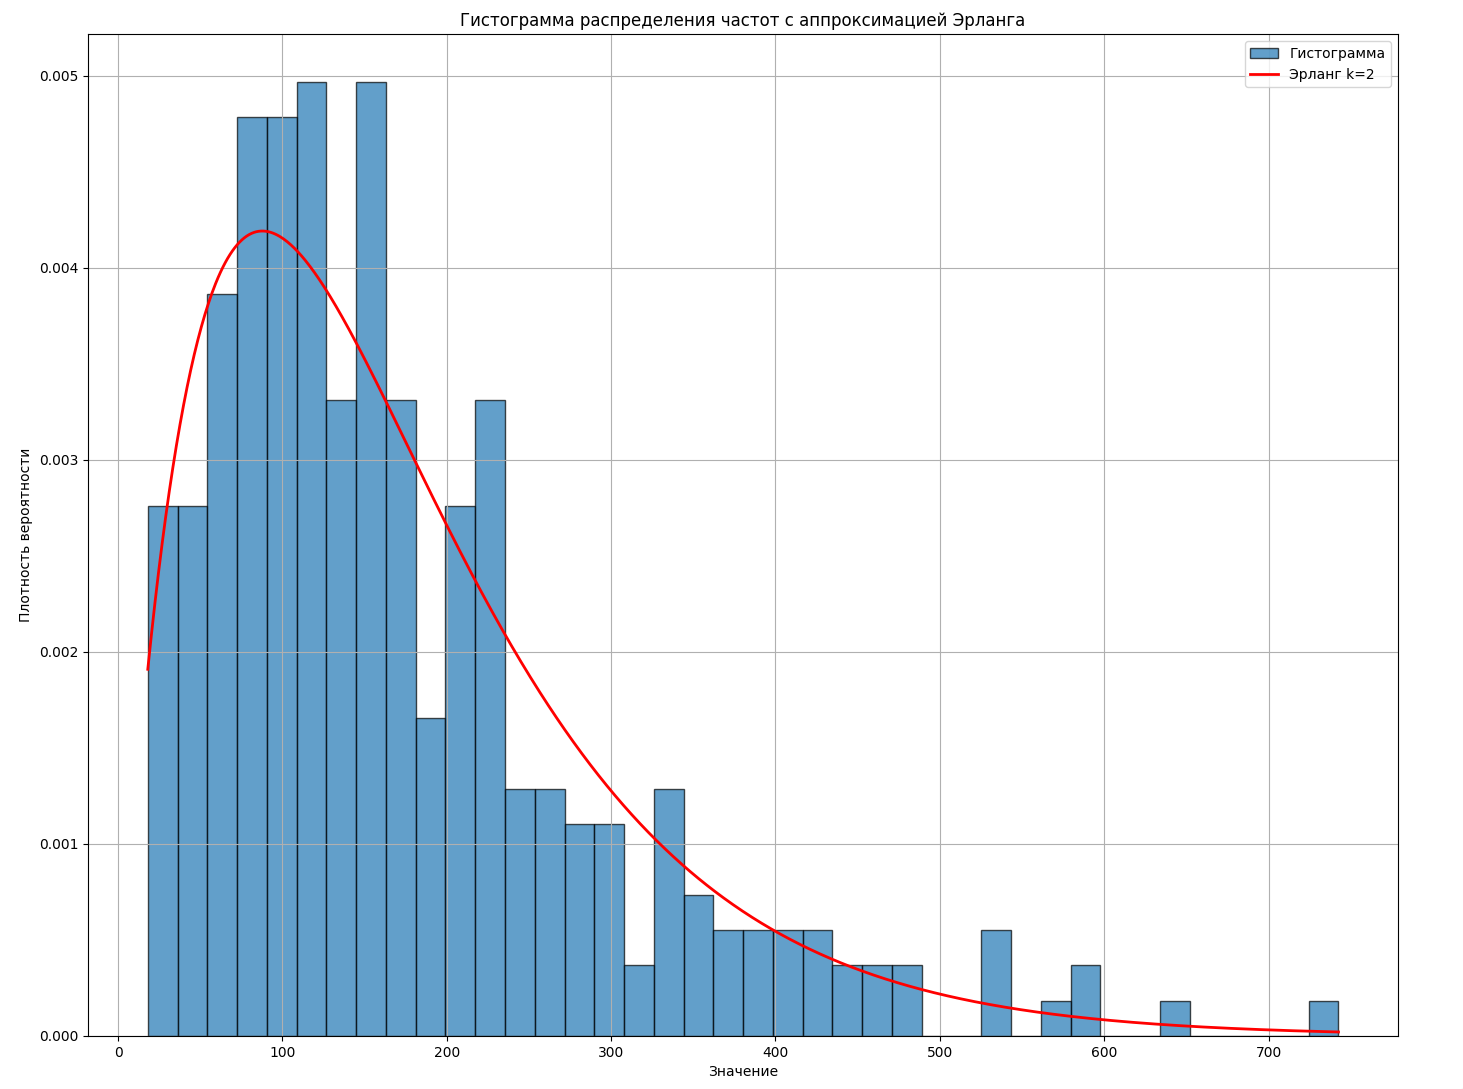
\includegraphics[width=1\textwidth]{../data/histogram_approximated.png}
	\caption{Распределение Эрланга для различных параметров}
\end{figure}
\FloatBarrier

\subsection{Вывод}

Для каждого случая был рассчитан соответствующий параметр \(\lambda\), основанный на среднем значении подвыборок. Аппроксимация показала, что распределение соответствует нормированному закону Эрланга для значений коэффициента вариации.
